\begin{abstract}
As electronic devices get increasingly personalized,
mixed signal integrated circuits such as analog to digital converters (ADCs)
and digital to analog converters (DACs) play a pivotal role in interfacing 
between the real world and the digital domain. Side-by-side, the security
requirements of these devices are increasing manifold. Many of these devices
require to be authenticated and have built in techniques to support 
encryption and prevent counterfeiting. For embedded devices, 
these requirements are efficiently implemented by 
using physically unclonable functions (or PUFs) that make use of the 
unique nanoscale variations during device fabrication.

In this paper, we show how mixed signal ICs in a device like ADCs and DACs 
have properties that make them amicable for use in PUF applications. By
virtue of having analog components, the PUF properties in these ICs
are significantly more amplified compared to digital PUFs such as those based on
SRAM and ring oscillators. An added advantage is that mixed signal PUFs
have considerably less overheads compared to the contemporary digital PUFs. 
\end{abstract}

\section{Introduction}
The physical characteristics of every electronic device is unique.
The uniqueness is due to micro and nanoscale variations in the 
silicon substrate and fabrication process. A physically unclonable function 
(or PUF) uses this uniqueness to provide a cryptographic key that 
cannot be forged. PUFs have wide application, especially for device
authentication, anti-counterfeiting, and tamper resistance.

Several PUFs have been constructed over the years. Most of them
from electronic components such as the SRAM, ring oscillators, flip flops,
FPGA units etc. A few non-electronic PUFs such as optical, acoustic,
and magnetic PUFs have also been proposed. The important requirements
for a PUF is that they should be compact, unforgeable, unpredictable, 
irreversible, reliable, and easy to evaluate. These requirements are 
easier said than met. Many of the requirements are contrasting, while 
many are drastically affected by noise and other environmental factors 
such as the ambient temperature. Thus the search for the search for 
the perfect PUF is an open problem and active area of research.

We propose to construct PUFs using mixed-signal components such as {\em analog to
digital converters} (ADCs) and {\em digital to analog converters} (DACs).
As their names suggest, ADCs convert analog voltage signals 
to equivalent digital data, while DACs convert digital data into the corresponding
analog voltage. These devices are omnipresent in embedded 
systems such as mobile phones, wireless sensor nodes, smart tablets, etc.
and are often integrated into micro-controllers~\cite{xxx}. 
In mobile phones for instance, DACs are used to sample audio signals and convert
them into the digital domain, while ADCs to drive the phone's speaker. 

Both ADCs and DACs have analog as well as digital parts. This is
appealing for constructing PUFs due to the following reasons.
\begin{itemize}
\item As ADCs and DACs have digital parts that are interfaced with the
processor, the resulting PUFs built from them are intrensic and  
directly accessible by applications running in the system. No external 
measuring equipment is required.

\item By virtue of having analog components in mixed-signal devices, 
micro and nano scale variations are likely to be observed in two dimensions : 
device delays and voltage levels. Compare this with the contemporary intrensic
PUFs, where the variations are only in one dimension; either in the delays or
the voltage level. For instance, in delay based PUFs like the arbiter and the 
ring oscillator PUF, inherient differences
only in delays are captured. On the other hand in memory based PUFs, memories 
cells settling to either 0 or 1 is captured. In comparison, there are multiple 
values an analog voltage can take.

\item MS-PUFs do not require any dedicated circuits on chip. It reuses ADCs and
DACs that are present in the microprocessor. Thus MS-PUFs do not have any overheads.
\end{itemize}

\begin{figure}[!b]
\centering
\caption{Mixed-Signal PUF in a Micro-controller with built-in ADC and DAC. }
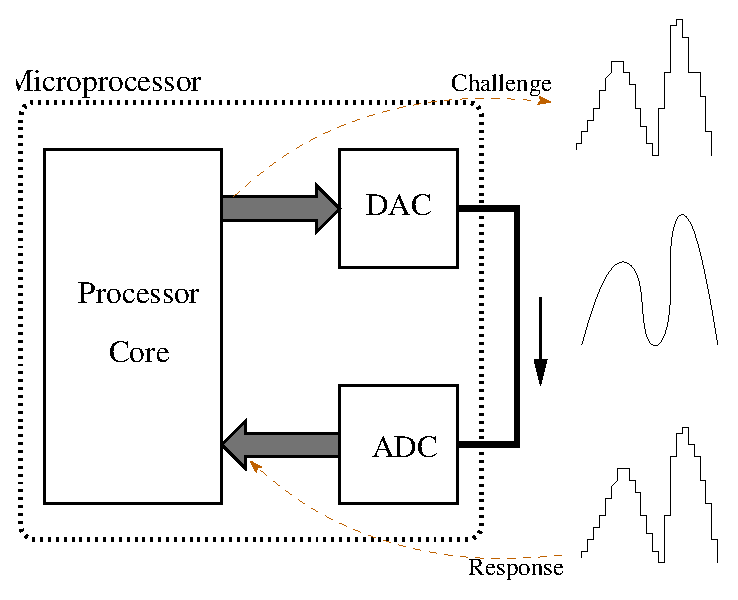
\includegraphics[width=6cm]{figs/mspuf}
\end{figure}


The scheme for the MS-PUF is shown in Figure~\ref{fig:mspuf}. An output of a DAC channel
is connected to the input of the ADC. A {\em challenge} in the form of a
digital time-series pattern is transferred to the DAC from the processor. This signal is
converted to analog at the DAC's output. The ADC quantifies and reconverts the signal 
into a time-series digital pattern. This ADC output is the {\em response} to the challenge.
Since the ADC and DAC are accessible from the processor, a software program can create 
create a challenge and read the corresponding response. 
The response is affected by many factors including the quantification and environmental
noise, and inherient variations due to the fabrication variations of the ADC and the 
DAC. The latter aspect is the focus for constructing the PUF.




The paper \ldots


The structre of the paper is as follows....

%\bibliographystyle{abbrv}
%\bibliography{screfs}

\section{Background}
\subsection{Physically Unclonable Functions}
A PUF relies on the fact that two similar devices tend to exhibit
different behaviour because of differences in their physical microstructure
and process variations during manufacture. A PUF extracts these 
differences by a 
series of challenges and responses. Each response is a 
function of the challenge and the device characteristics. Thus each device will
have a different response for the same challenge. A collection of challenge-response pairs
are used for several cryptographic applications such as device fingerprinting, 
authentication, anti-cloning, and generation of cryptographic keys.


The PUF's challenge and response can be represented by a function $f$ 
mapping the domain of challenges ($\mathcal C$) to a range of responses ($\mathcal R$).
\begin{equation*}
f : \mathcal C \rightarrow \mathcal R \,\,\,
  | \,\,\, f(c) = r, \text{ where } c \in \mathcal C \text{ and } r \in \mathcal R
\end{equation*}

The function $f$ should be one-way, easy to evaluate and reproduce, yet unpredictable
and unclonable. 

\subsection{Mixed Signal Circuits}
Mixed signal circuits interface the analog and digital domains in a chip. 
They are typically used to digitalize real world signals captured by
a sensor, which
can then be processed by software. They are also used to actuate external 
hardware devices. 
For instance, in a mobile phone, audio signals captured from 
a microphone are digitalized by means of an {\em analog to digital converter
(ADC)}, before being processed by the mobile software. Received audio data is
converted to analog by a {\em digital to analog converter (DAC)} and actuate the
speakers of the mobile phone. This section provides the necessary background
for ADCs and DACs.

{\flushleft \em Digital to Analog Converters.}
An $n$-bit DAC converts an $n$-bit digital value into a corresponding analog
voltage. A typical DAC uses an R-2R network as shown in Figure~\ref{fig:r2r}.
Each stage in the network comprises of a pair of 
resistors (R and 2R) and a switch $s_i$ 
($0 \le i \le n$). The switch $s_i$ is closed only if the $i$-th bit of the
digital data is one. The resulting voltage at the amplifier's input is the
sum of voltages due to each closed switch. 
Each switch contributes a voltage of $\frac{1}{2^{n-i}}$, 
where $n < i \le 0$. 
Thus, the analog voltage at the amplifier's input
is proportional to the digital data.

\begin{figure}
\includegraphics[width=6cm]{SA-ADC.png}
\centering
\caption{Block diagram of a 4-bit R-2R DAC\label{fig:r2r}}
\end{figure}

{\flushleft \em Analog to Digital Converters.}
An $n$-bit ADC converts an analog voltage (or current) to 
an equivalent $n$-bit digital data. The commonly used ADCs are
flash, successive-approximation, and sigma-delta ADCs. We give
a brief background on the successive-approximation ADC; the 
ADC we used for our expermients.

A successive-approximation ADC {\em SA-ADC} converts an analog
input to digital using a binary search technique.
In SA-ADC, a successive approximation register(SAR) containing 
a digital value is fed to an internal DAC and its output is 
compared to the input voltage. A sample and hold(SAH) circuit 
is used to supply constant input voltage to the comparator. 
A SA-ADC provides medium levels of accuracy and conversion time. 
The PUF output variation can occur because of microscopic variations 
in electrical components used in SAH circuit and internal DAC.
%It suffers from thermal noise for capacitors($kT/C$) which increases with temperature and is inversely proportional to the capacitance. However with higher capacitance, power consumption increases and accuracy decreases and usually a trade off is required.


\section{Mixed Circuit PUFs}
Nano scale variations in DACs and ADCs.





A R-2R DAC suffers from thermal noise which increases with resistance and temperature. The PUF output variation can occur because of microscopic variations in the resistors and switches used.


two people speaking through a mobile phone. Sound is converted to an analog signal by the microphone, which is
then converted to digital form by an analog to digital converter(ADC) for transmission. In the other end, the digital
data is converted to analog by a digital to analog converter(DAC) and the speaker converts to audible sound. In this
digitalizing world, ADC and DAC modules are omnipresent in all devices. The main reason behind this is that all the input from
the external world is analog in nature and the device process everything digitally. This factor plays a key role in
the idea of using ADC and DAC components for PUFs. The ADC and DAC modules can be embedded inside the chip or outside the chip.

A set of hexadecimal values is passed to the DAC which converts it to its corresponding analog values which is again fed to ADC which converts back to digital value. So our challenge is an array of digital values which is fed to the DAC and response is calculated from the digital values output by the ADC of the device.The microscopic variations present in the ADC and DAC components gives rise to an unique response for each device for the same set of challenges. This mixed circuit based PUF is cost effective and very efficient as it does not require expensive hardware like arbiters and oscillators for digital electronic PUFs and can be easily reproducible unlike non electronic PUFs. Moreover, ADC and DAC components are ubiquitous in modern digital devices and can be modified easily with little effort and integrated effortlessly into the current crop of devices.



\section{Evaluation}




\section{Related Works}
In the last decade various types of PUFs have been proposed. The PUFs are categorized into either
electronic PUFs or non-electronic PUFs. Electronic PUFs are further classified into analog-electronic
PUFs and digital-intrinsic PUFs. The various types of PUFs are discussed in this section.

\subsection{Non-electronic PUFs}
As the name suggests, non-electronic PUFs use randomness arising due to non electronic components in the system
such as from optical, acoustic, and magnetic media. In the case of \textit{Optical PUFs} for instance, the main 
component is an optical token which is doped with refractive glass spheres in a random fashion. When the token is 
radiated with a laser, a speckle pattern is formed. The patterns are  unique because  of the microscopic differences 
between the tokens. In \textit{Acoustic PUFs}, mechanical vibrations is the main source of
randomness. The vibrations causes a sound wave, which scatters yielding unique reflections. 
Non-electronic PUFs do not have wide usability due to expensive hardware and accurate positioning 
required for their construction.

\subsection{Analog electronic PUFs}
In these PUFs, partial randomness introduced due to electronic quantities like capacitance or 
resistance is measured. 
For example, in a \textit{power distribution PUF}, voltage drops based on resistance variations
in the power grid of a chip is measured. The voltage drops are partial random owing to the
variations in manufacturing. In a \textit{V\_T PUFs}, differences due to manufacturing variations
on the threshold voltage of transistors is exploited. In both these PUFs external measuring instruments
are required, making them expensive.


\subsection{Digital Intrinsic PUFs}
The PUFs discussed so far are non-intrinsic, where randomness is explicitly introduced into the
system. In intrinsic PUFs, the challenge response 
collection mechanism is embedded in the device. There are two types of intrinsic PUFs :
delay-based and memory-based. In delay-based PUFs, random delays in propagating a current signal
through wires is exploited. Commonly used delay-based PUFs are arbiter PUFs and ring oscillator 
PUFs. In memory-based PUFs, randomness in settling of values in memory cells is exploited. 
These include SRAM PUFs, Butterfly PUFs and Flip-flop PUFs.



\section{Conclusion}
